\section{Background}\label{sec:background}
\label{sec:cast}
The Gauss-Bonnet Theorem states

\begin{equation} \label{eqn:g-b}
\sum_{v\in V_{int}} K(v) + \sum_{v\in V_{\partial S}} k_g(v) = 2\pi \chi(S).
\end{equation}
In this section, we define these symbols.


\subsection{Simple Polygons}
\label{sec:warm-up}

To get a sense of the types of problems we will encounter,
we begin by deriving a formula for the area
of a simple polygon on the sphere in terms of the 
interior angles.
\begin{theorem}\label{thm:triangle}
In the plane, the sum of the interior angles of a triangle is $\pi$.
\end{theorem}
\begin{proof}
Draw a line parallel to one edge through the opposite vertex.
By alternating interior angles in the plane, the sum of the angles
in the triangle equal  a straight line.
See \figref{angles} for an illustration. 



\begin{figure}[htb]
\centering
\includegraphics[width=.3\textwidth]{background/interior-angles-triangle}
\caption{A proof that, in the plane, the sum of the angles of a triangle is $\pi$.}
\label{fig:angles}
\end{figure}

\end{proof}



Consider any simple polygon in the plane $P$ with $n$ vertices. 
Then $P$ can be triangulated with $n-2$ triangles \cite{orourke_computational_1994}.
Thus, when we traverse $P$ we go around $n-2$ triangles each contributing
$\pi$.
We have
\begin{corollary}\label{cor:angles}
In the plane, any simple polygon $P$ with $n$ vertices,
the sum of the interior angles of $P$ is $(n-2)\pi$.

\end{corollary}

Now consider a triangle on the two dimensional sphere as in \figref{sphere-triangle}.

\begin{figure}[htb]
\centering
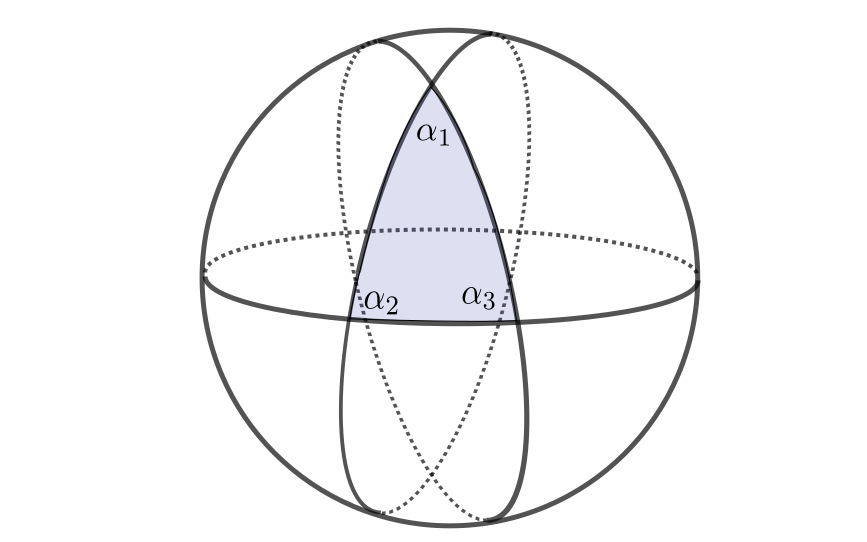
\includegraphics[width=.5\textwidth]{background/sphere-triangle}
\caption{A triangle on the sphere.}
\label{fig:sphere-triangle}
\end{figure}


\begin{figure}[htb]
\centering
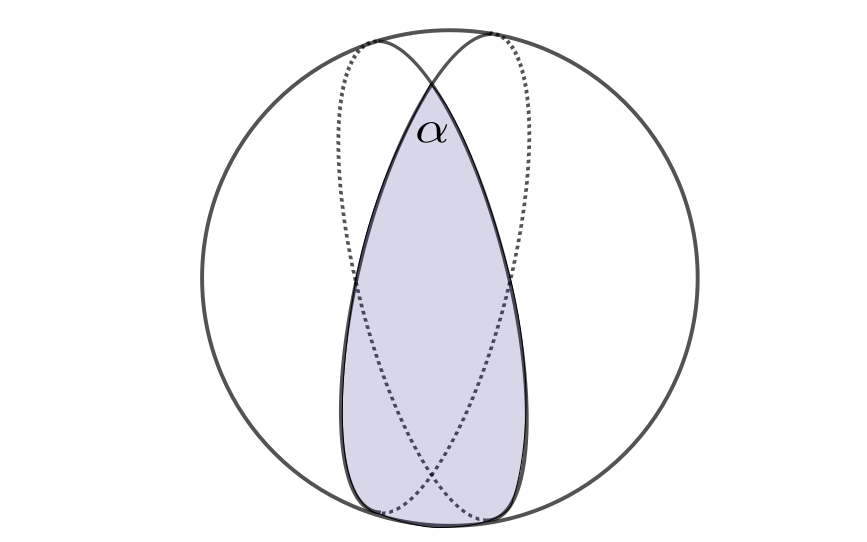
\includegraphics[width=.4\textwidth]{background/lune}
\caption{A lune with angle $\alpha$.}
\label{fig:lune}
\end{figure}




\subsection{Triangulations}

Here we define simplicial complexes and triangulations.
Most introductory topology texts has contain these definitions \cite{munkres,jm08}.

\begin{definition}[Topological Space \cite{munkres}]
A \EMPH{topology} is a pair $(X,\tau)$, where $X$ is a set and
 $\tau$ is a collection of subsets $X$
satisfying:
	\begin{itemize}
		\item $\emptyset$ and $X$ are in $\tau.$
		\item the union of \emph{any} subcollection of elements in $\tau$ is  in $\tau.$
		\item the intersection of any \emph{finite} subcollection of elements in the $\tau$ is in $\tau.$
	\end{itemize}
A set $X$ with a specified topology $\tau$ is called a \EMPH{topological space}.
\end{definition}

We will work with a special type of topological spaces called manfiolds.

\begin{definition}[Manifold  \cite{tu2011}]
	A topological space $M$ is \EMPH{locally Euclidean of dimension $n$}
	if every point $p$ in $M$ has a neighborhood $U$ such that there is  a
	homeomorphism  $\phi$ from $U$ into and open  subset of $\R^n$.
	We call the pair $(U,\phi: U\to \R^n)$ a \EMPH{chart}, $U$ a \EMPH{coordinate neighborhood}
	and  $\phi$ a \EMPH{coordinate map}. 
A \EMPH{manifold} is a Hausdorff, second countable, locally Euclidean space.
\end{definition}

We will  consider two and three dimensional manifolds. Two dimensional
manifolds are called \emph{surfaces}.
The symbol $S$ in \eqnref{g-b} is a surface.
In order to perform computations on our manifolds, 
we often want a triangulation of our manifolds.
To define triangulations we need some preliminary definitions.



\begin{definition}[Independent Points]
Let $v_0,v_1,\ldots,v_k$ be points in $\R^n$. We call them \EMPH{affinely dependent}
if there are real numbers $\alpha_0,\alpha_1,\ldots,\alpha_k$, not all 0, such that
$\Sigma_{i=0}^k \alpha_iv_i=0$ and $\Sigma_{i=0}^k \alpha_i=0.$
Otherwise,  $v_0,v_1,\ldots,v_k$ are \EMPH{affinely independent}.

\end{definition}

\begin{definition}[Simplices]
A \EMPH{simplex} $\sigma$ is the convex hull of a finite affinely independent
set $A$ in $\R^n$. The points in  $A$ are  called vertices, the dimension
of  $\sigma$ is $|A|-1$.  The convex hull of a subset of vertices of a simplex
$\sigma$ is a \EMPH{face} of $\sigma$.
\end{definition}

\begin{definition}[Simplicial Complex]
A nonempty family $C$ of simplices is a \EMPH{simplicial complex} if the following
are satisfied:
\begin{itemize}
\item  Each face of any simplex is a simplex.
\item The intersection of $\sigma_1 \cap \sigma_2$ is a face of both $\sigma_1$ and 
$\sigma_2$.
\end{itemize}


\end{definition}

Some simplicial complexes are very similar to others.


\begin{definition}[Homeomorphism]
A  \EMPH{homeomorphism}  of topological spaces $(X_1,\tau_1$ and $(X_2,\tau_2)$
is a bijection $\phi:X_1\to X_2$ such that for every $\phi$ and $\phi^{-1}$ are continuous.
\end{definition}
For two topological spaces $X$ and $Y$ if there exists a  homeomorphism between
$X$ and $Y$ we say $X$ and $Y$ are topologically  equivalent and write  $X\cong Y.$

Manifolds can have a boundary denoted $\partial(M)$.
The dimension of $\partial(M)$ is one less than the dimension of $M$ .
We are ready to define a triangulation.

\begin{definition}[Triangulation]
For a topological space $X$ and simplicial complex $C$ if $X\cong C$,
then $C$  is a \EMPH{triangulation} of $X$.
\end{definition}

We denote the vertices, edges and faces of a triangulated surface as $V, E$ and $F$ respectively.
Let $V_{\partial}$ denote vertices on the boundary of a surface and let $V_{int}$ 
denote vertices that are not on the boundary.
See \figref{triangulated-torus} for an example of a triangulated surface.
Often, it is useful to approximate smooth surfaces with fine triangulations called
a \emph{mesh}. We will see meshes in many of our applications.


\begin{figure}[htb]
\centering
\includegraphics[width=.3\textwidth]{curvature/triangulated-torus}
\caption{A triangulation of the torus.}
\label{fig:triangulated-torus}
\end{figure}

\subsection{Curvature}

There are several ways to define curvature in the discrete setting \cite{Crane:2013}.
We present two of them here. 




For a vertex in a discrete surface, the Gaussian curvature is defined as
follows

\begin{definition}[Discrete Gaussian curvature]\label{def:discrete-curvature-vertex}

The discrete \EMPH{Gaussian curvature} at a vertex $v$ is the area on the unit sphere bounded by a spherical polygon whose vertices are the unit normals of the faces around $v$.

\end{definition}


\begin{figure}[htb]
\centering
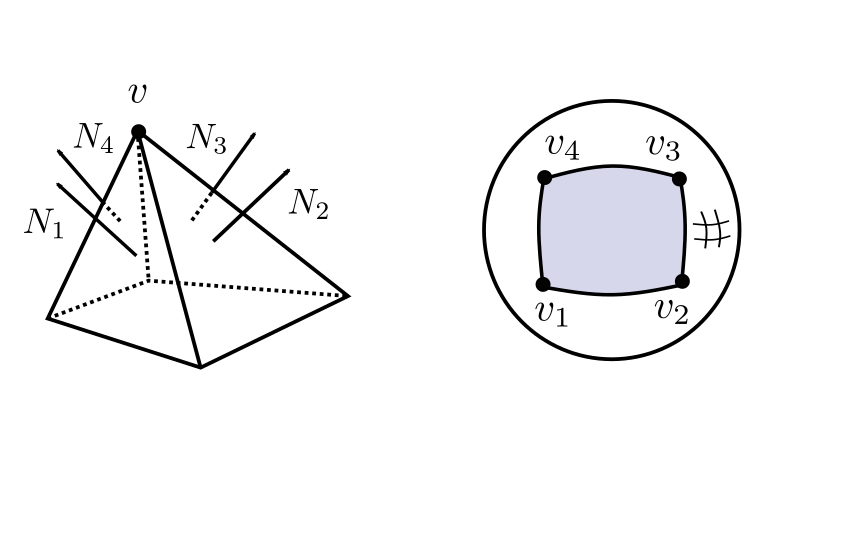
\includegraphics[width=.3\textwidth]{curvature/discrete-curvature}
\caption{The discrete curvature at vertex $v$ is the area drawn on the sphere.}
\label{fig:discrete-curvature}
\end{figure}


\corref{sphere-area} gives a formula for computing the curvature at a vertex, provided
we know the interior angles of the polygon on the sphere.
The interior angles of the polygon $\beta_i$ on the sphere are supplementary to
the angle $\alpha_i$ incident to $v$ in the surface

\begin{equation} \label{eqn:switcheroo}
\beta=\pi-\alpha.
\end{equation}
See \figref{switcheroo} for an example.




\begin{figure}[htb]
\centering
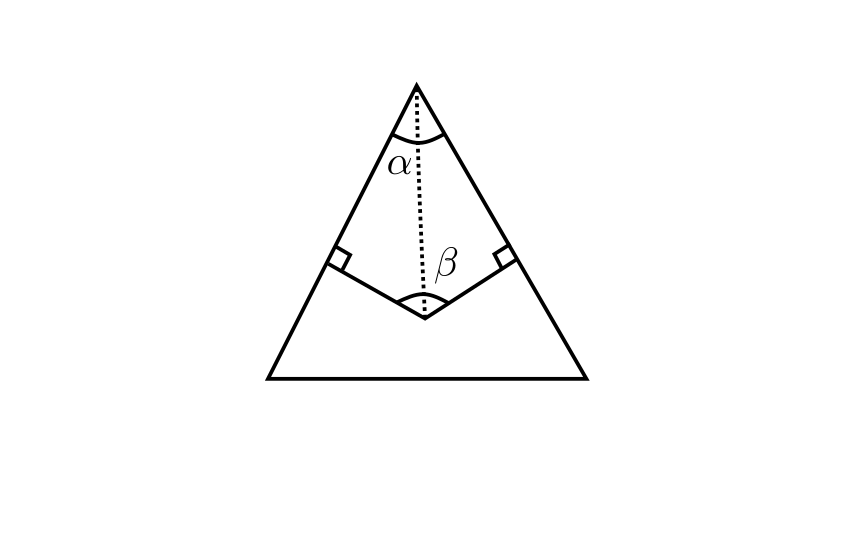
\includegraphics[width=.3\textwidth]{background/switch-angles}
\caption{The relationship between the angles incident to a vertex and
the interior angles of the area polygon on the sphere.}
\label{fig:switcheroo}
\end{figure}




This gives a convenient formula for computing the curvature at a vertex.
The \EMPH{angle defect} at a vertex $d(v)$ is the difference between $2\pi$ and
the sum of the incident angles.  Let $F_v$ denote the faces containing $v$  
and let $\alpha_f$  denote the interior  angle of face $f$ at $v$, then
$$d(v):=2\pi -\sum_{f\in F_v}\alpha_f.$$

Since $\beta_i=\pi-\alpha_i$, we have the Gaussian curvature at $v$
is 
$$k(v)=2\pi -n\pi+\sum_{i}^n \beta_i=2\pi-n\pi +n\pi -\sum_i^n\alpha_i=d(v)$$
 and the
 angle defect is equal to the discrete curvature in \defref{discrete-curvature-vertex}.


For a vertex $v$ on the boundary of a surface, we define the the curvature
of $v$  to be 
$$k_{\partial}(v)= \pi-\sum_{f\in F_vi}\alpha_f.$$
Notice that if $v$ lies on a straight line, then $\sum_{i}\alpha_f=\pi$
and the curvature is $0$ as we would expect.
For historical reasons,  we write $k_g(v)=k_{\partial}(v)$
where the subscript $g$ refers to geodesic curature.
Curvature is defined more naturally in the continuous setting,
discrete curvature is an oxymoron.  See do Carmo \cite{doc76} for an introduction.
The juxtaposition between the continuous and discrete versions of the theorem
is pleasing.





\subsection{The Euler Characteristic}

Properties of topological spaces that remain unchanged by homeomorphisms are called
\EMPH{topological invariants}. One such invariant is the Euler characteristic.
Originally defined for polyhedra, the \EMPH{Euler Characteristic} for surfaces $\chi$ is the 
the number of vertices minus the number of edges plus  the number of faces, $\chi=V-E+F.$
In higher dimensions, for a triangulated space $X$ the Euler characteristic is 
$\chi(X)=k_0-k_1+k_2-k_3+\ldots$ where $k_n$ is the number of simplices of dimension $n.$
A  graph  is \EMPH{planar} if it can be drawn in the plane with intersections only occuring
at vertices.
For a planar graphs $V-E+F=2$, Eppstein maintains a collection of proofs of this \cite{eppstein-proofs}.
We include the the following proof from Eppstein's list attributed to Thurston
 \cite{thurston}. For any planar graph we can map the graph on to the two sphere
 using stereographic projection.
 
\begin{theorem}[Euler Characteristic for Planar Graphs]\label{thm:euler}
For any planar graph on the 2-sphere we have $V-E+F=2.$
\end{theorem}

\begin{proof}
If needed, perturb the triangulation so that the north and south poles are 
inside of a two faces and there are no vertical edges. At each vertex place a unit positive
charge, at the center of each edge place a unit negative charge and put a unit positive
charge in the middle of each face. Slam the sphere on the ground so that all charges
on the edges and vertices are moved into the face below them. For faces that do not contain a pole
the net charge will be zero, the northern boundary consists of an alternating sequence
of edges and vertices  beginning  and ending with an edge.
The face containing the north pole has a unit positive charge, and the face containing the south
pole contains positive four units of charge and negative three units of charge.
Thus, the total charge is two.

\end{proof}

The \EMPH{genus} of a surface is the maximum  number of closed simple
non-intersecting curves that can be drawn in the surface without separating
the surface.
The torus in \figref{triangulated-torus} has genus two.
By the classification of surfaces, the Euler characteristic or an orientable surface
is determined by its genus with $\chi=2-2g$.

Putting all of these variables together gives \eqnref{g-b}.
The  Gauss-Bonnet theorem is  telling us, if we add up curvature
at each vertex the sum will be $2\pi$ times to Euler characteristic.
If we can compute the curvature at every vertex then we can use the theorem
to learn global topological information.
Conversely, if we know the Euler characteristic we can learn about the curvature
at individual points.
